%\VignetteIndexEntry{Sushi}
\documentclass{article}
\title{Sushi: An R/Bioconductor package for visualizing genomic data}
\author{Douglas H Phanstiel, Alan Boyle, Carlos Araya, and Mike Snyder}
\usepackage{Sweave}
\begin{document}
\Sconcordance{concordance:Sushi.tex:Sushi.Rnw:%
1 4 1 1 0 2 1 1 5 39 1 1 2 1 0 2 1 3 0 1 2 2 1 1 2 13 0 1 2 8 1 1 2 13 %
0 1 2 5 1 1 2 1 0 3 1 4 0 1 2 4 1 1 2 4 0 1 2 1 6 1 2 6 1 1 2 1 0 1 1 3 %
0 1 2 1 8 1 2 4 1 1 2 1 0 2 1 1 2 1 0 1 3 2 0 1 1 4 0 1 2 5 1 1 3 2 0 1 %
2 1 0 1 4 5 0 1 20 1 3 5 1 1 2 4 0 1 2 4 1 1 3 2 0 2 1 1 2 4 0 1 2 3 1 %
1 18 1 2 4 1 1 3 2 0 1 1 1 2 1 0 1 1 3 0 1 2 3 1 1 37 1 2 6 1 1 2 13 0 %
1 2 4 1 1 2 1 0 2 1 1 2 1 0 1 2 1 0 1 1 4 0 1 2 9 1 1 2 1 0 2 1 1 3 1 0 %
1 3 1 0 1 2 4 0 1 2 7 1 1 2 20 0 1 2 4 1 1 2 1 0 2 1 1 3 2 0 1 1 1 2 1 %
0 2 1 4 0 1 2 5 1 1 2 1 0 2 1 1 3 2 0 1 1 1 2 5 0 1 2 7 1 1 2 13 0 1 2 %
3 1 1 2 1 0 2 1 1 4 2 0 1 2 1 3 5 0 1 2 4 1 1 2 1 0 2 1 1 4 2 0 1 2 1 3 %
5 0 1 2 4 1 1 2 1 0 2 1 1 4 2 0 1 7 5 0 2 2 4 0 1 2 4 1 1 2 1 0 2 1 1 4 %
2 0 1 7 5 0 2 2 4 0 1 2 4 1 1 2 1 0 4 1 1 3 1 0 1 4 2 0 1 2 1 4 2 0 2 2 %
4 0 1 2 7 1 1 2 13 0 1 2 4 1 1 3 2 0 4 1 4 0 1 2 20 1 1 2 1 0 1 1 3 0 1 %
2 2 1 1 2 1 0 2 1 1 3 1 0 2 2 1 1 3 0 1 2 2 1 1 10 1 2 3 1 1 2 1 0 1 1 %
1 2 1 1 3 0 1 2 1 1 1 19 1 2 3 1 1 3 2 0 1 3 1 0 3 1 1 3 1 0 1 3 1 0 3 %
1 3 0 1 2 2 1 1 39 1 3 3 1}

\maketitle
\section{Introduction}

Sushi is an R package for plotting genomic data stored in multiple common genomic formats including bed, bedpe, bedgraph format. The flexible code allows for integration of the plots into multipanel figures that can include plots made by sushi, R basecode, or other R packages.  Sushi allows for simple flexible plotting of gene structures, transcript structures, sequencing tracks, ChIP seq peaks, chromatin interactions, GWAS results and other commen genomic data types.   


\section{Example datasets}
To illustrate how Sushi works, we have included several publicaly available data sets in the package Sushi. The data types include RNA-seq, ChIP-seq, ChIA-PET, and HiC data and can be loaded using the following commands

\begin{Schunk}
\begin{Sinput}
> library('Sushi')
> Sushi_data = data(package = 'Sushi')
> data(list = Sushi_data$results[,3]) 
\end{Sinput}
\end{Schunk}

\section{plotManhattan}

Manhattan plots can be plotted given SNPS and significance values in bed format.  The 'plotManhattan' function is used to plot the data while the 'labelgenome' function is used to add the genome labels to the x-axis.

\begin{center}

\begin{Schunk}
\begin{Sinput}
> # make color palette
> palette_fire_dark = colorRampPalette(c("black","blue","#5900E5","#E5001B","orange"))
> # make the plot
> plotManhattan(bedfile=Sushi_GWAS.bed,pvalues=Sushi_GWAS.bed[,5],genome=Sushi_hg18_genome,col=palette_fire_dark(nrow(Sushi_hg18_genome)),cex=0.75)
> # add labels
> labelgenome(genome=Sushi_hg18_genome,side=1,scipen=20,n=4,scale="Mb",edgeblankfraction=0.20,line=.18,chromline=.5,scaleline=0.5)
\end{Sinput}
\end{Schunk}
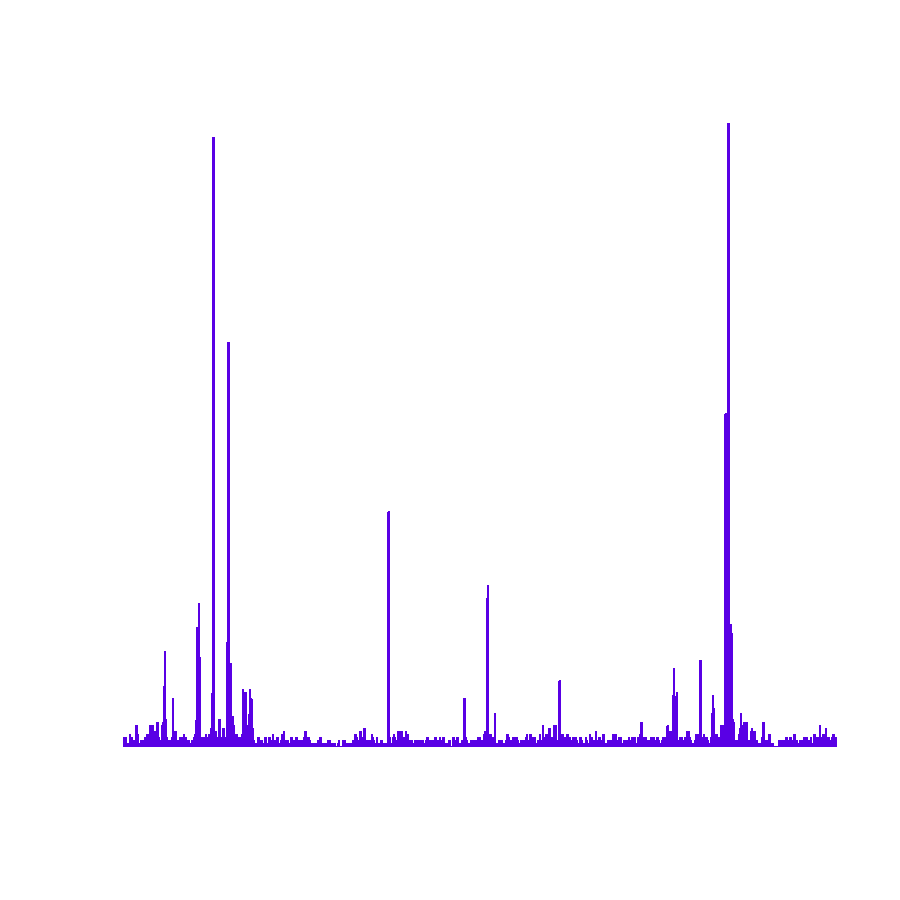
\includegraphics{Sushi-002}
\end{center}
\end{document}


